\section{Real Time Clock}

A Phase-Locked Loop (PLL) operates by synchronizing the frequency of a Voltage-Controlled Oscillator (VCO) with that of an input signal.
\begin{figure}[H]
    \centering
    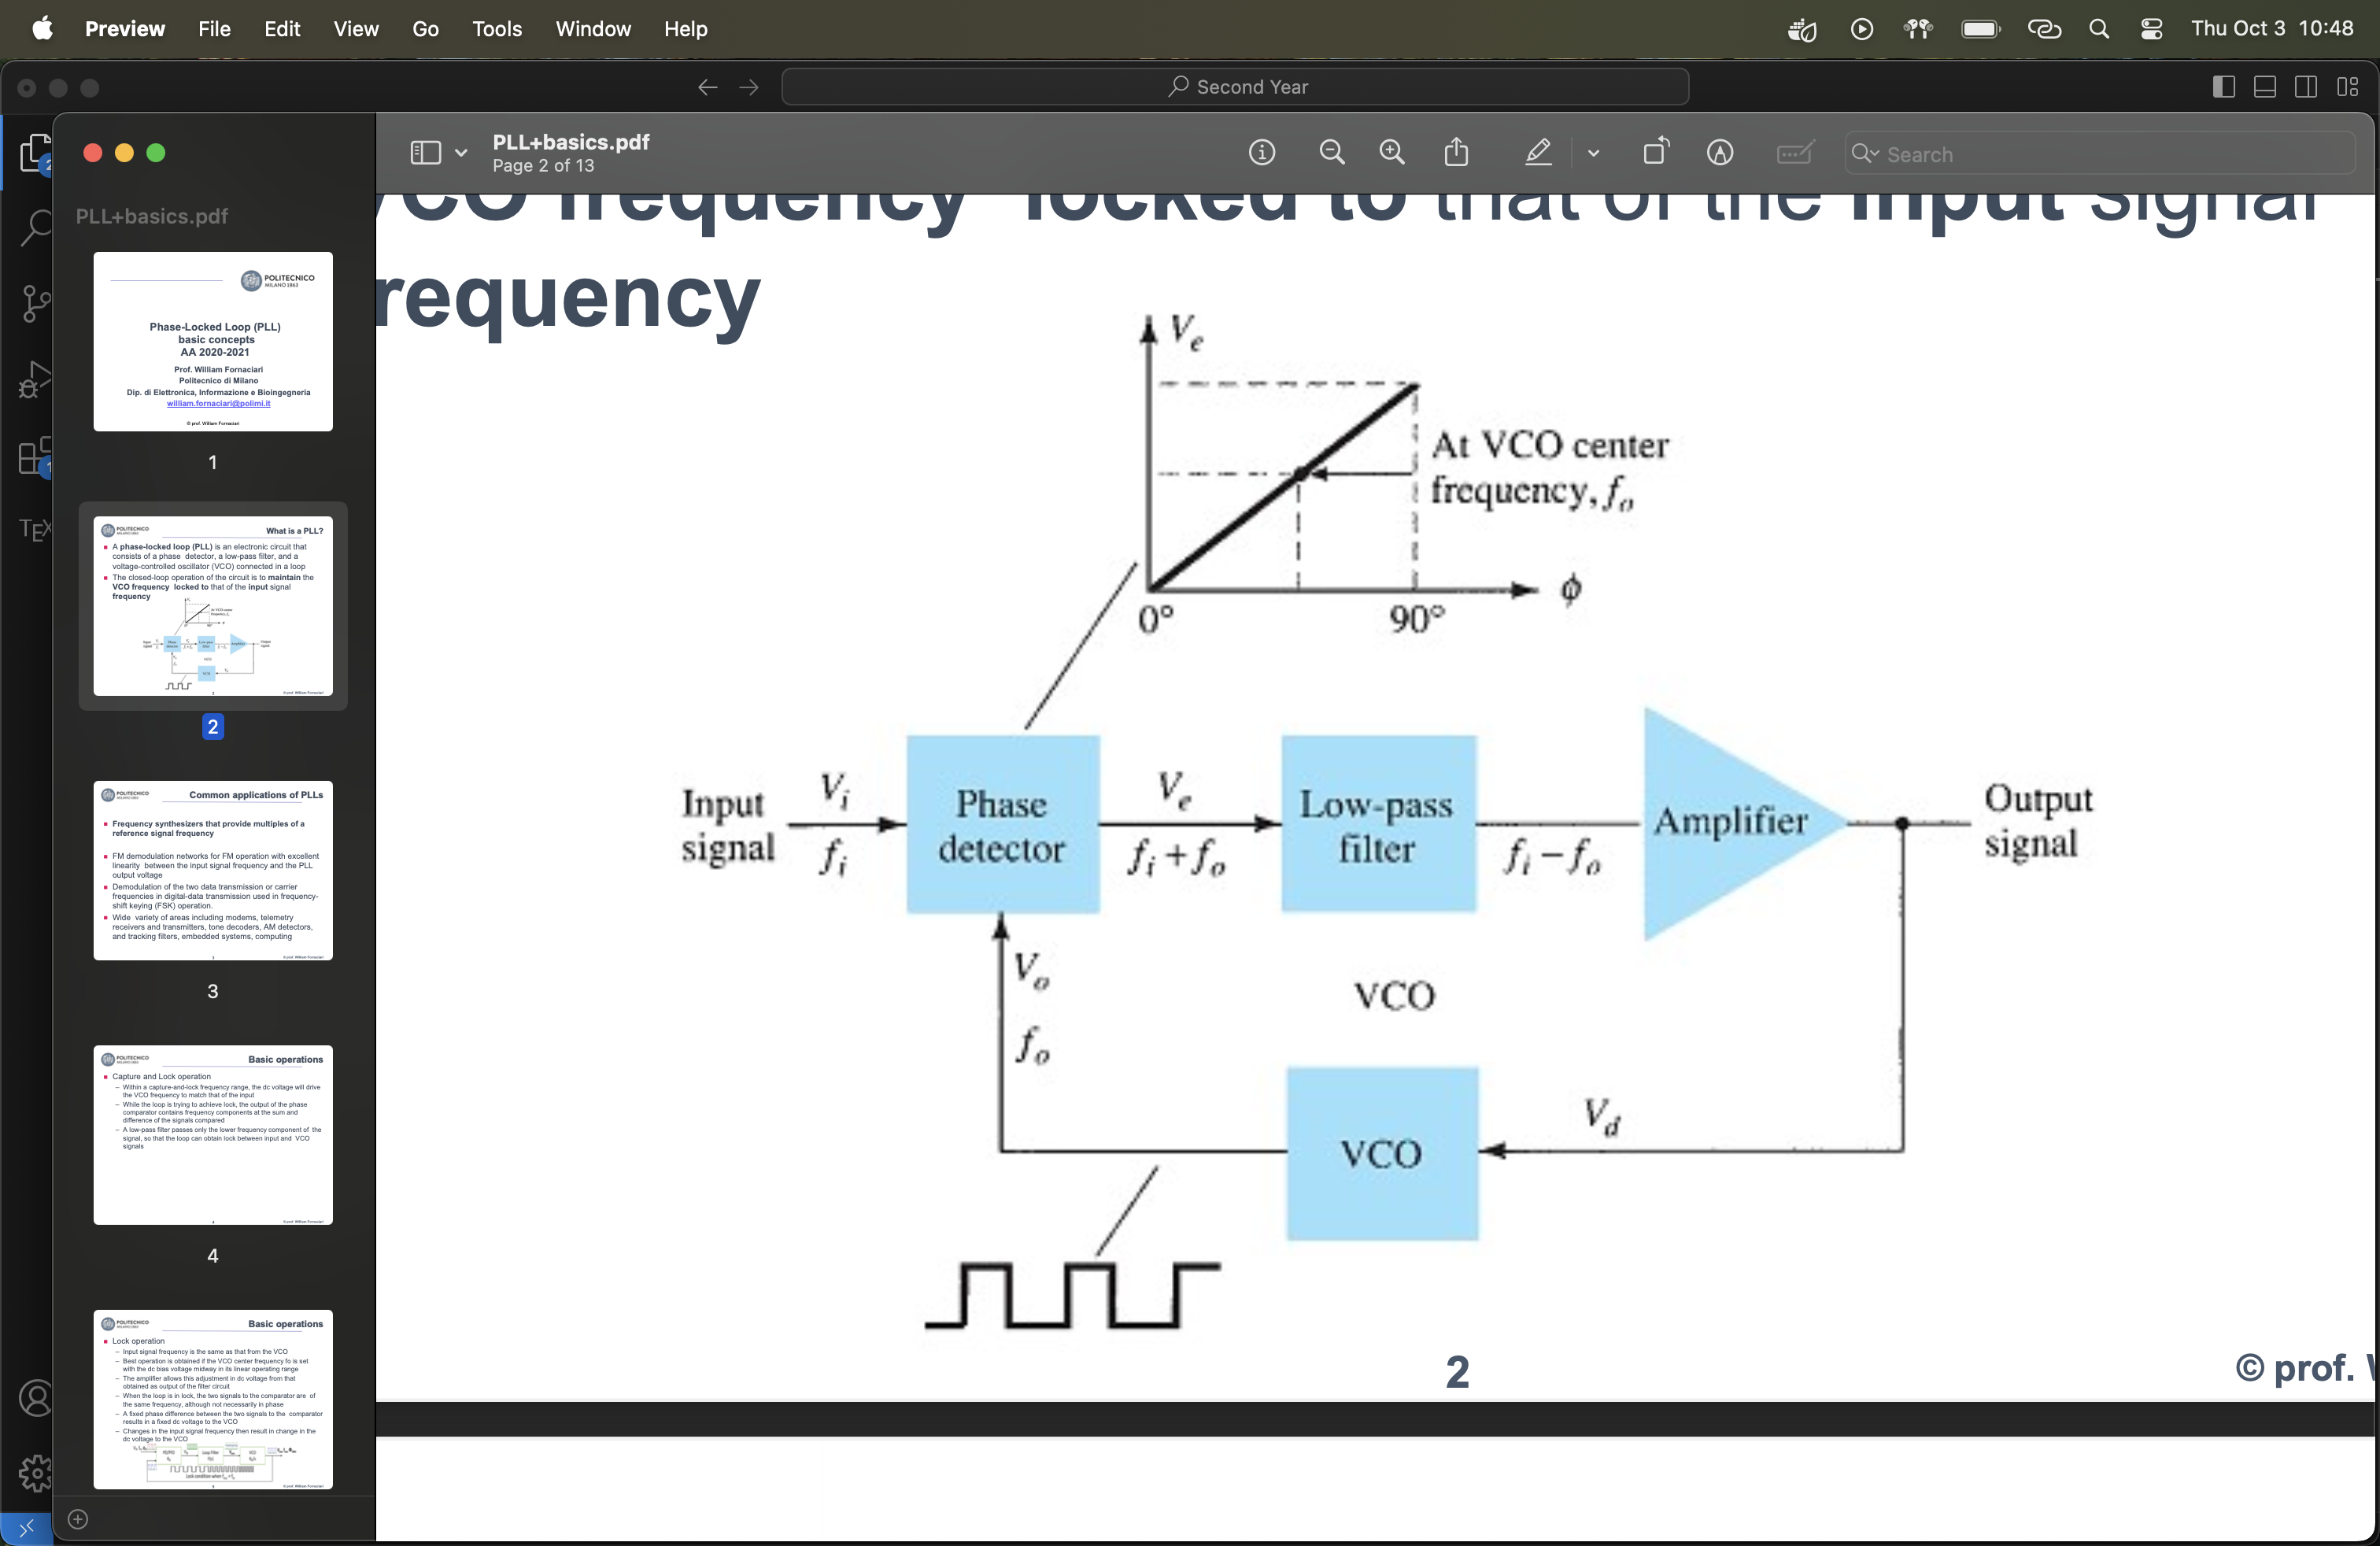
\includegraphics[width=0.75\linewidth]{images/pll.png}
    \caption{Phase-Locked Lopp}
\end{figure}
In normal operation, when the loop is locked, the input and VCO output frequencies are identical. 
The phase detector generates a fixed phase difference between these signals, which is converted into a DC control voltage applied to the VCO. 
As the input signal frequency fluctuates, the phase detector adjusts this DC voltage to maintain synchronization.
We have two useful frequencies in a PLL:
\begin{itemize}
    \item \textit{Capture range}: the frequency range around the VCO's free-running frequency within which the PLL can initially acquire lock with the input signal.
    \item \textit{Lock range}: once the PLL is locked, it can maintain synchronization with the input signal over a wider frequency range than the capture range. 
\end{itemize}
The main applications of a PLL include:
\begin{itemize}
    \item \textit{Clock multiplier} or \textit{clock generator}: generates a clock signal that is a multiple of the input frequency or provides multiple clock outputs.
    \item \textit{Frequency synthesizer}: produces a clock signal with an arbitrary frequency by dividing or multiplying a reference clock.
        A frequency divider is placed between the VCO output and the phase comparator. 
        The output frequency is divided down before being feedback to the phase detector. 
        As long as the loop remains locked, the VCO output will be an integer multiple of the input frequency. 
        \begin{figure}[H]
            \centering
            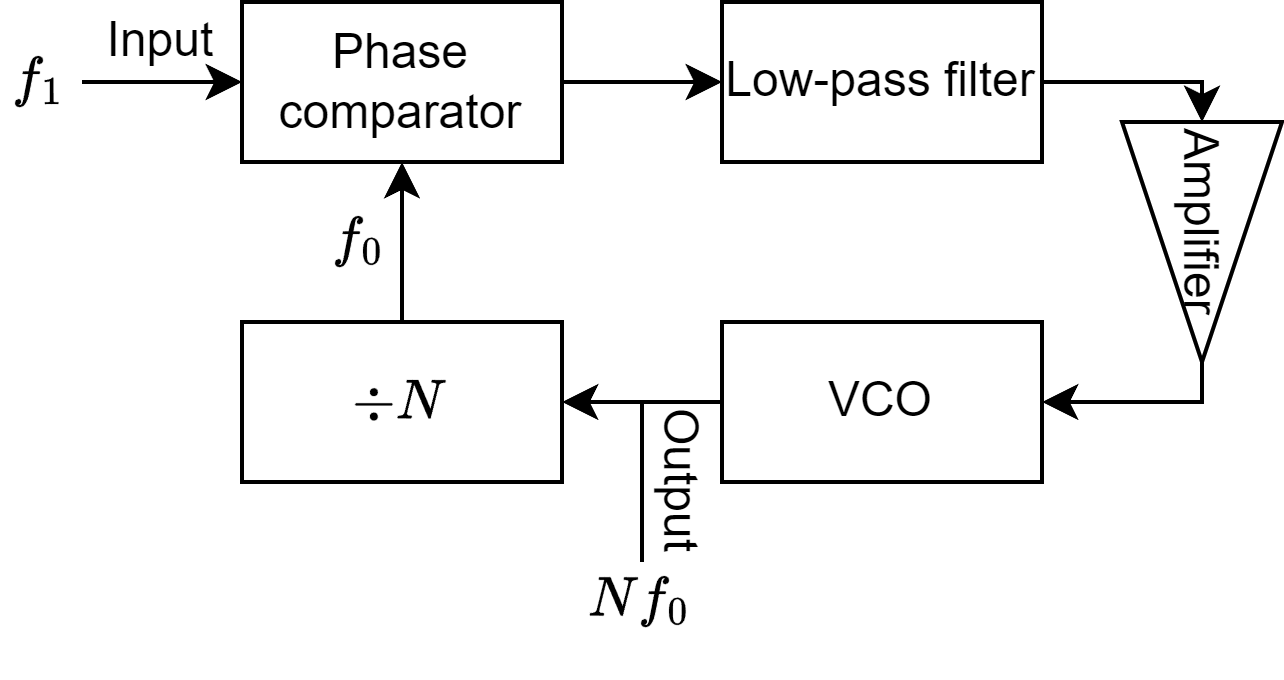
\includegraphics[width=0.65\linewidth]{images/freq.png}
            \caption{Frequency synthesizer}
        \end{figure}
    \item \textit{Clock and data recovery}: recovers digital data and a synchronized clock signal from a serial data stream, using a specialized phase detector.
    \item \textit{Frequency and module demodulation}: demodulates a radio signal by tracking the frequency modulation and converting it into a usable signal.
\end{itemize}

\paragraph*{Integer synthesizer}
An integers-N synthesizer is created by using a stable, high-frequency crystal oscillator and divide its output.
The output frequency $f_{{o}}$ can be expressed as:
\[f_{{o}}=f_{\text{ref}}\dfrac{n}{r}\]
Here, $f_{\text{ref}}$ is the reference frequency, $n$ and $r$ are programmable integer values that can be selected based on system requirements.
\begin{figure}[H]
    \centering
    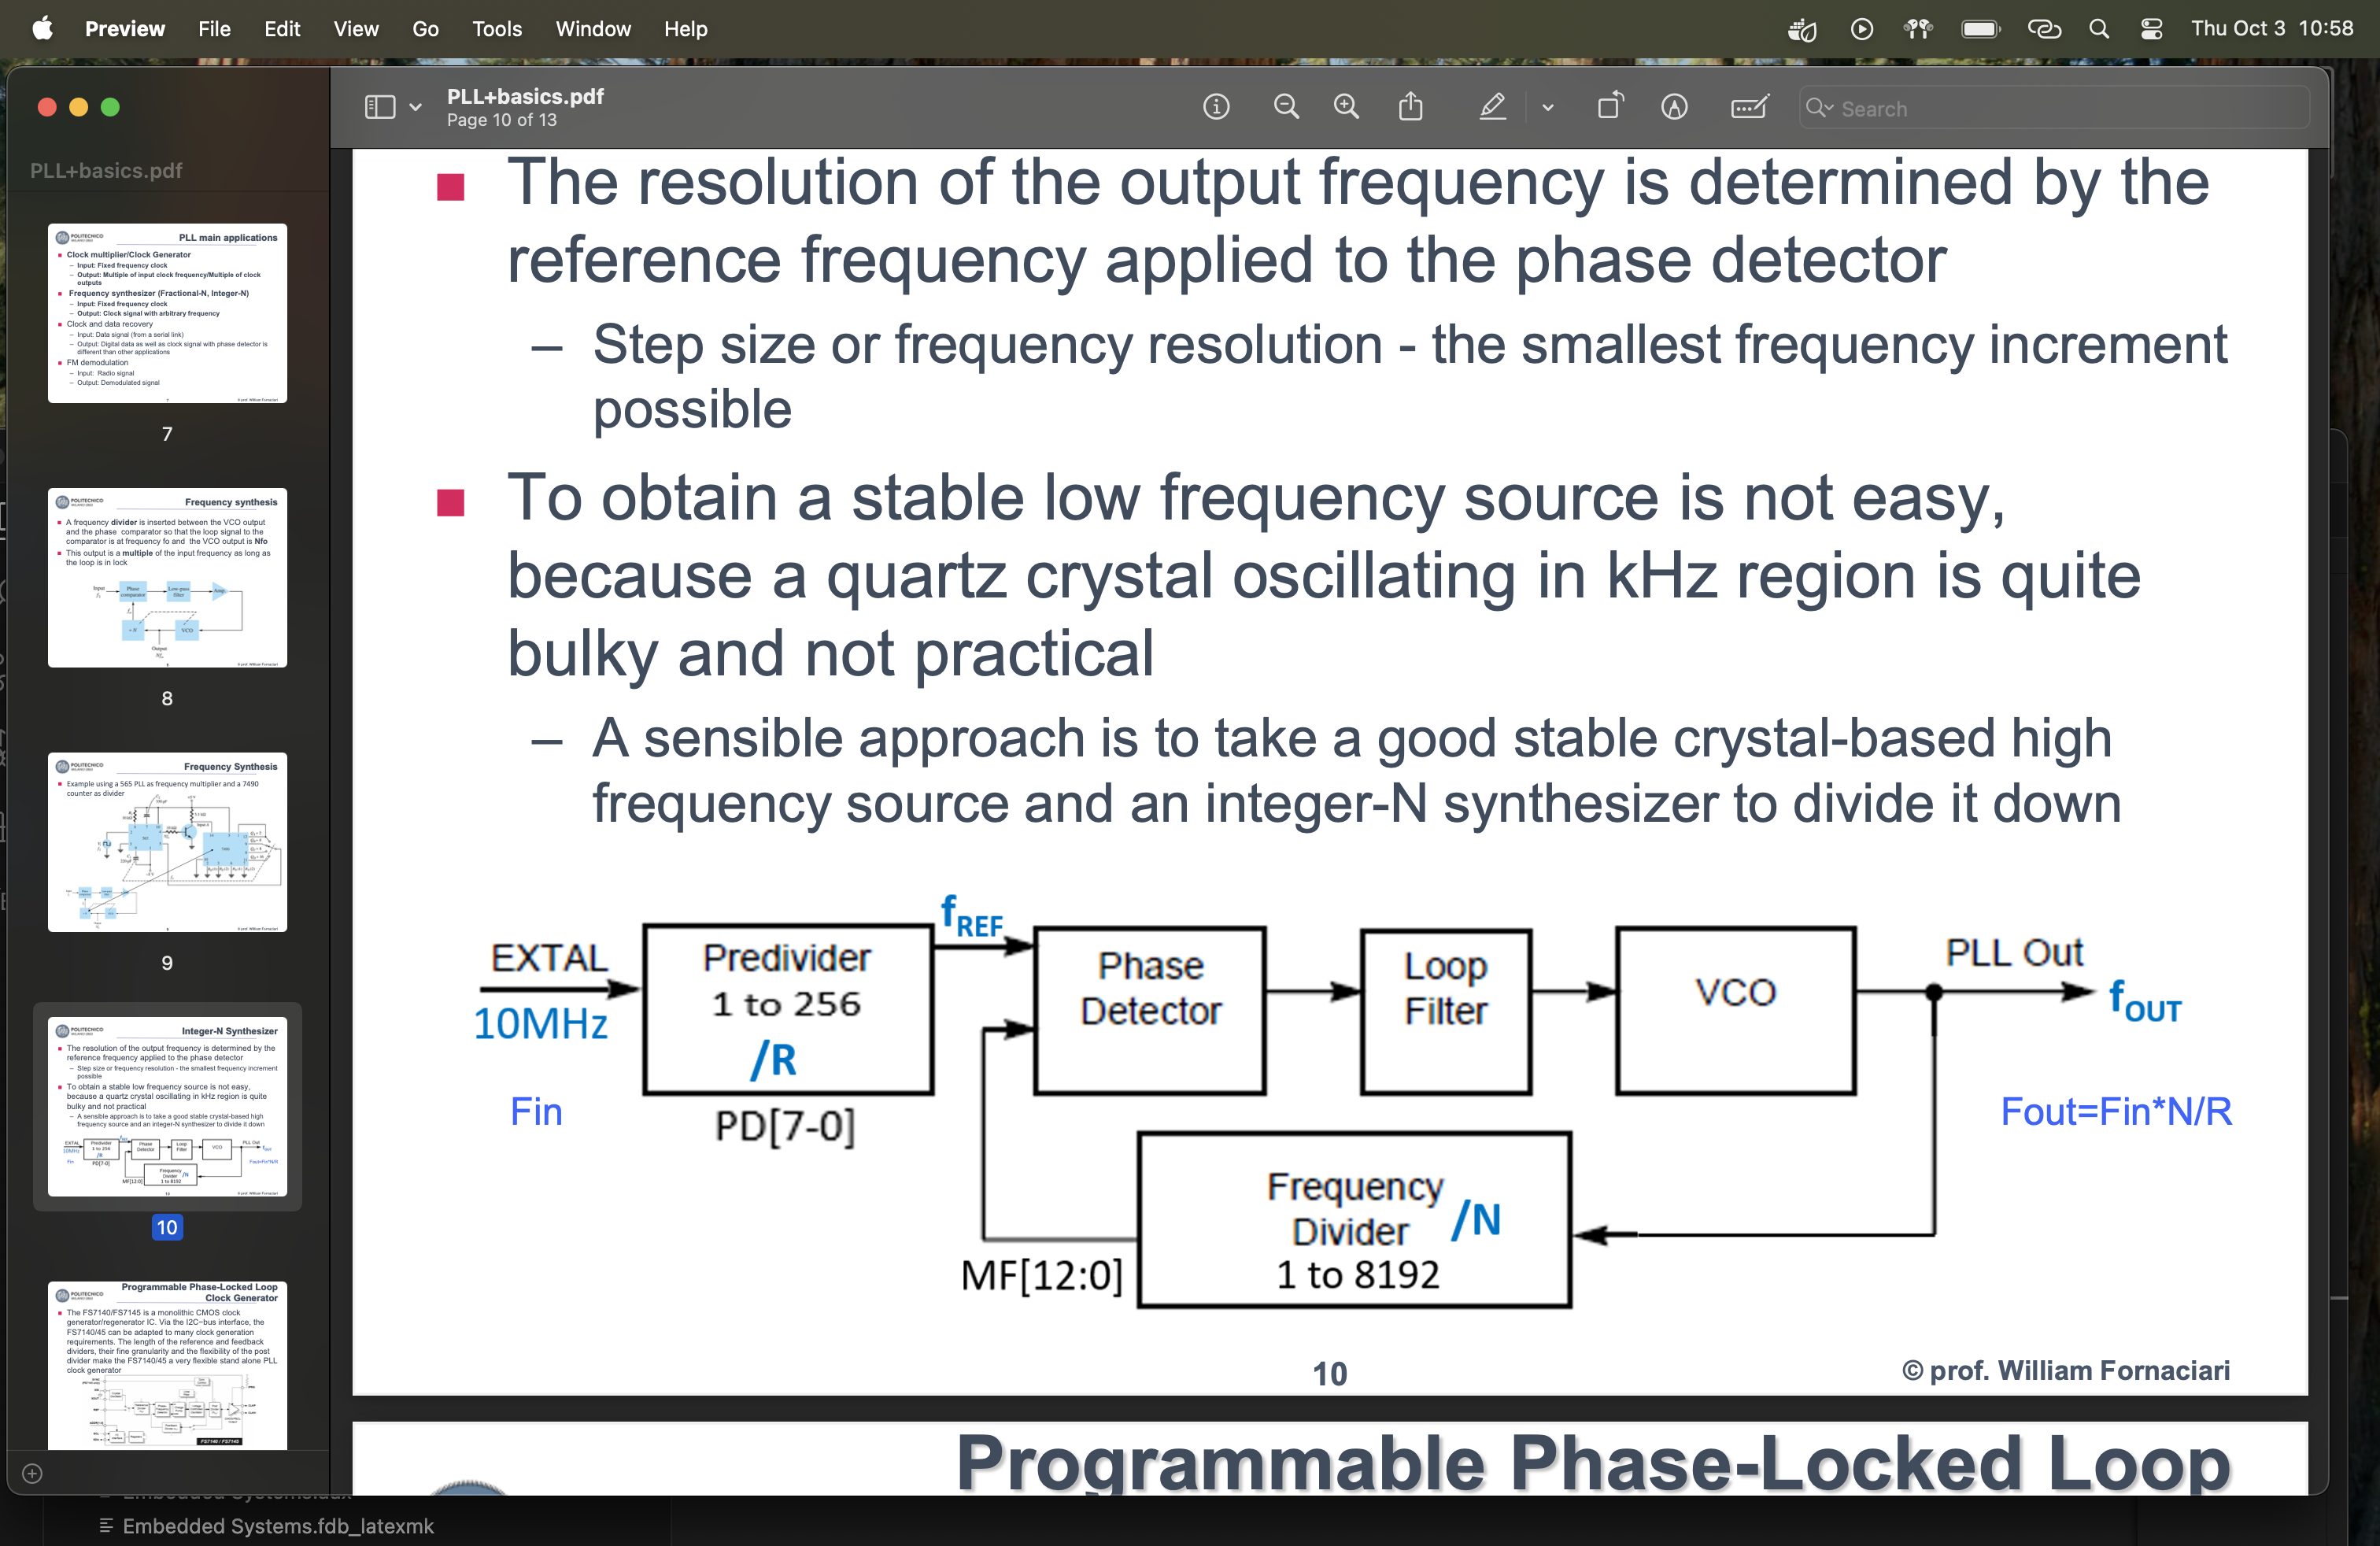
\includegraphics[width=0.75\linewidth]{images/freqn.png}
    \caption{Integer-N synthesis}
\end{figure}

\paragraph*{Prescalers}
Prescalers are frequency dividers that reduce the frequency of the VCO before it reaches the phase detector and extend the frequency range of a synthesizer. 
A four-modulus prescaler provides four scaling factors and uses two control signals to select one of the available factors. 
\begin{figure}[H]
    \centering
    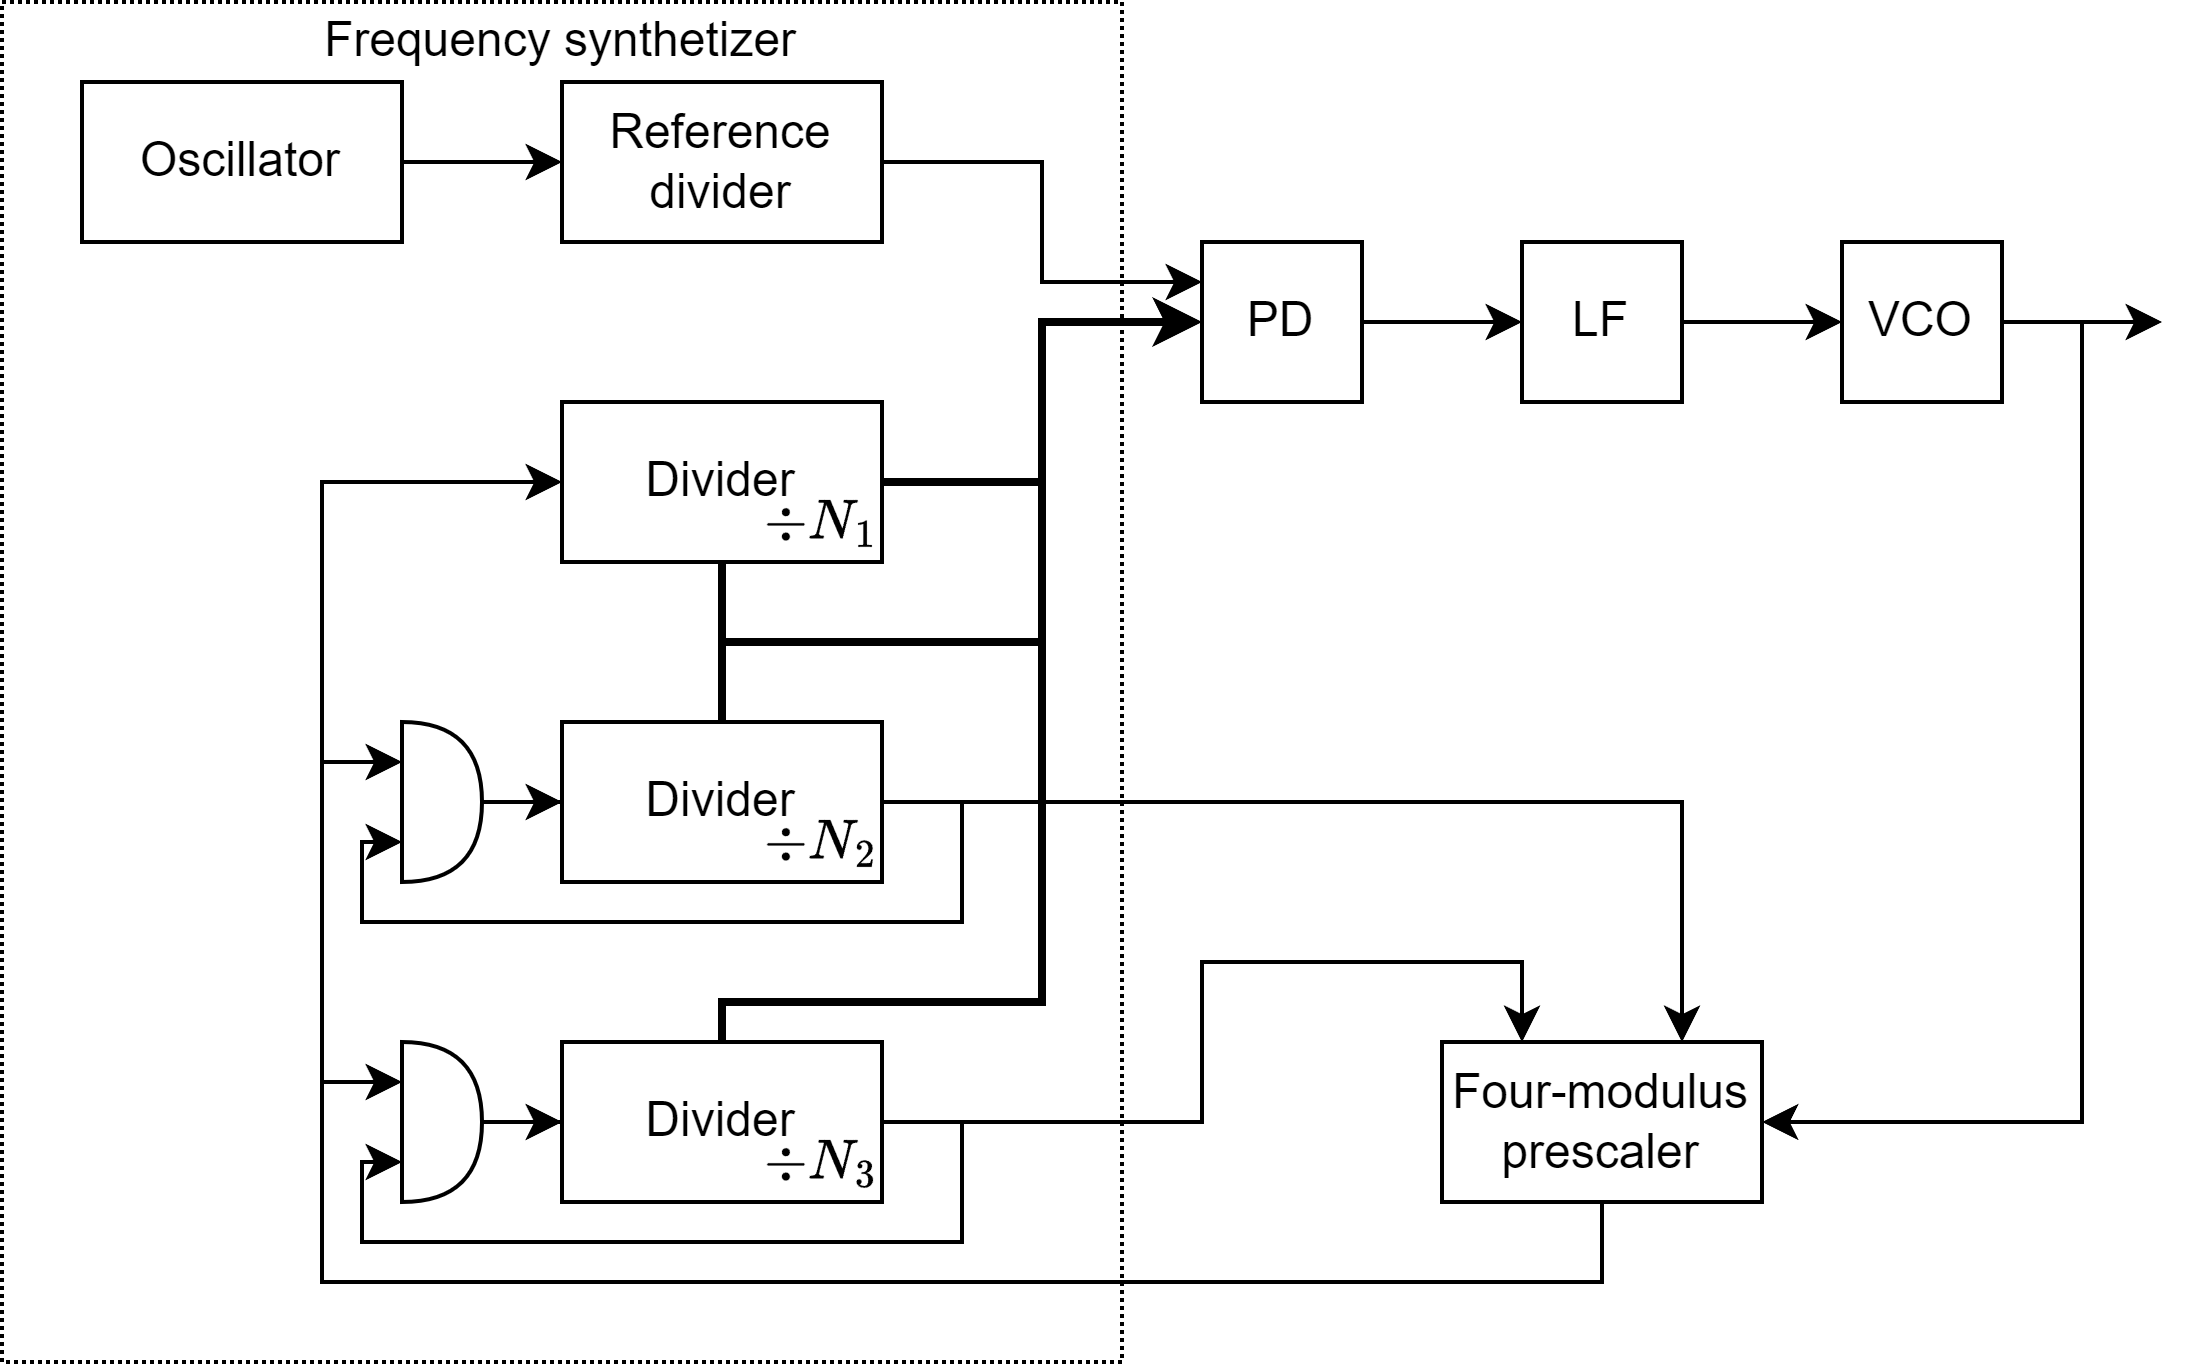
\includegraphics[width=0.75\linewidth]{images/freqp.png}
    \caption{Integer-N synthesis with prescalers}
\end{figure}
This design allows dynamic adjustment of clock speeds to optimize performance and power consumption.
By combining prescalers with PLLs, systems can adapt to variable computational loads while maintaining efficient power use.

\subsection{Timers}
A programmable timer is a specialized clock used to measure time intervals or count events. 
\begin{table}[H]
    \centering
    \begin{tabular}{|c|c|c|}
    \hline
    & \textbf{Timer} & \textbf{Counter} \\ \hline
    \textbf{Increment} & \makecell{The register is incremented \\ for every machine cycle} & \makecell{The register is incremented \\ based on a 1 to 0 transition \\ at an external input pin ($T_0, T_1$)} \\ \hline
    \makecell{\textbf{Maximum} \\ \textbf{count rate}} & $\frac{1}{12}$ of the oscillator frequency & $\frac{1}{24}$ of the oscillator frequency \\ \hline
    \textbf{Source of signal} &\makecell{A timer uses the frequency of the \\ internal clock to generate delay} & \makecell{A counter uses an external \\ signal to count pulses} \\ \hline
    \end{tabular}
\end{table}
Counters are similar to timers but are designed to count external events instead of clock cycles. 

\paragraph*{Registers}
Timers are controlled through some special function registers, such as: 
\begin{itemize}
    \item \textit{Gate}: the timer only runs while an external interrupt is active. 
    \item \textit{Start and stop control}: timers can be started and stopped via software or hardware control. 
    \item \textit{Counter or timer select bit}: this bit determines whether the module operates as a timer or a counter. 
\end{itemize}

\paragraph*{Reading}
There are two primary values to read from a timer:
\begin{itemize}
    \item \textit{Timer value}: read the actual count value stored in the timer registers. 
    \item \textit{Timer overflow}: monitor the timer overflow flag, which is set when the timer reaches its maximum value. 
\end{itemize}

\paragraph*{Settings}
Timers can be used to perform two main tasks: 
\begin{itemize}
    \item \textit{Polling}: continuously reading the status registers to check for timer events or the current counter value. 
        Polling can consume significant processing time and may introduce variability in response times, especially in complex programs.
    \item \textit{Interrupts}: generate an interrupt when a specific event occurs. 
        This method ensures fast and predictable responses to timer events, without requiring the main program to check for them continuously.
\end{itemize}

\paragraph*{Structure}
The basic structure of a timer in an microcontroller consists of several essential components:
\begin{itemize}
    \item \textit{Clock source}: multiple clock sources may be available, with the possibility of selecting an external clock if needed.
    \item \textit{Prescaler}: divides the input clock by a factor. 
    \item \textit{Main counter}: after the prescaler, the clock feeds into a main counter that increments or decrements depending on the timer mode.
    \item \textit{Modulus value}: the main counter's range is controlled by a modulus value, which can be programmed into a register.
    \item \textit{Control logic}: the control logic defines the operational mode of the timer. 
\end{itemize}
Based on the usage, the timers can be: 
\begin{itemize}
    \item \textit{Periodic}: generate repetitive events or ticks with a fixed period (determined by the modulus value). 
    \item \textit{Delay}: execute actions after a specific time interval has passed. 
        This function works by resetting the timer to zero and waiting for a defined number of ticks before triggering the desired action.
\end{itemize}

Timers and counters are some of the most critical peripherals in microcontroller designs, enabling a wide variety of functions that improve performance, reduce power consumption, and simplify designs. 
Timers and counters can be used in virtually any application to enhance performance, reduce power usage, or streamline design by replacing CPU-based operations with interrupt-driven tasks.
Many COTS microcontroller devices include built-in support for programmable timers.
Manufacturers provide development kits and reference designs tailored to specific applications that rely heavily on programmable timers.

\subsection{Watchdog timer}
A watchdog timer detects software anomalies and takes corrective actions to recover from system faults, ensuring reliability.
Watchdog timers can be implemented as either external chips or integrated within the microcontroller itself. 
They may offer fixed or programmable timeout intervals. 

In normal operation, the system regularly kicks or resets the watchdog timer to prevent it from reaching its timeout. 
If a hardware fault or software error occurs, the system may fail to reset the timer and the watchdog will time out and generate a corrective action.
Corrective actions may vary depending on the fault.
\begin{figure}[H]
    \centering
    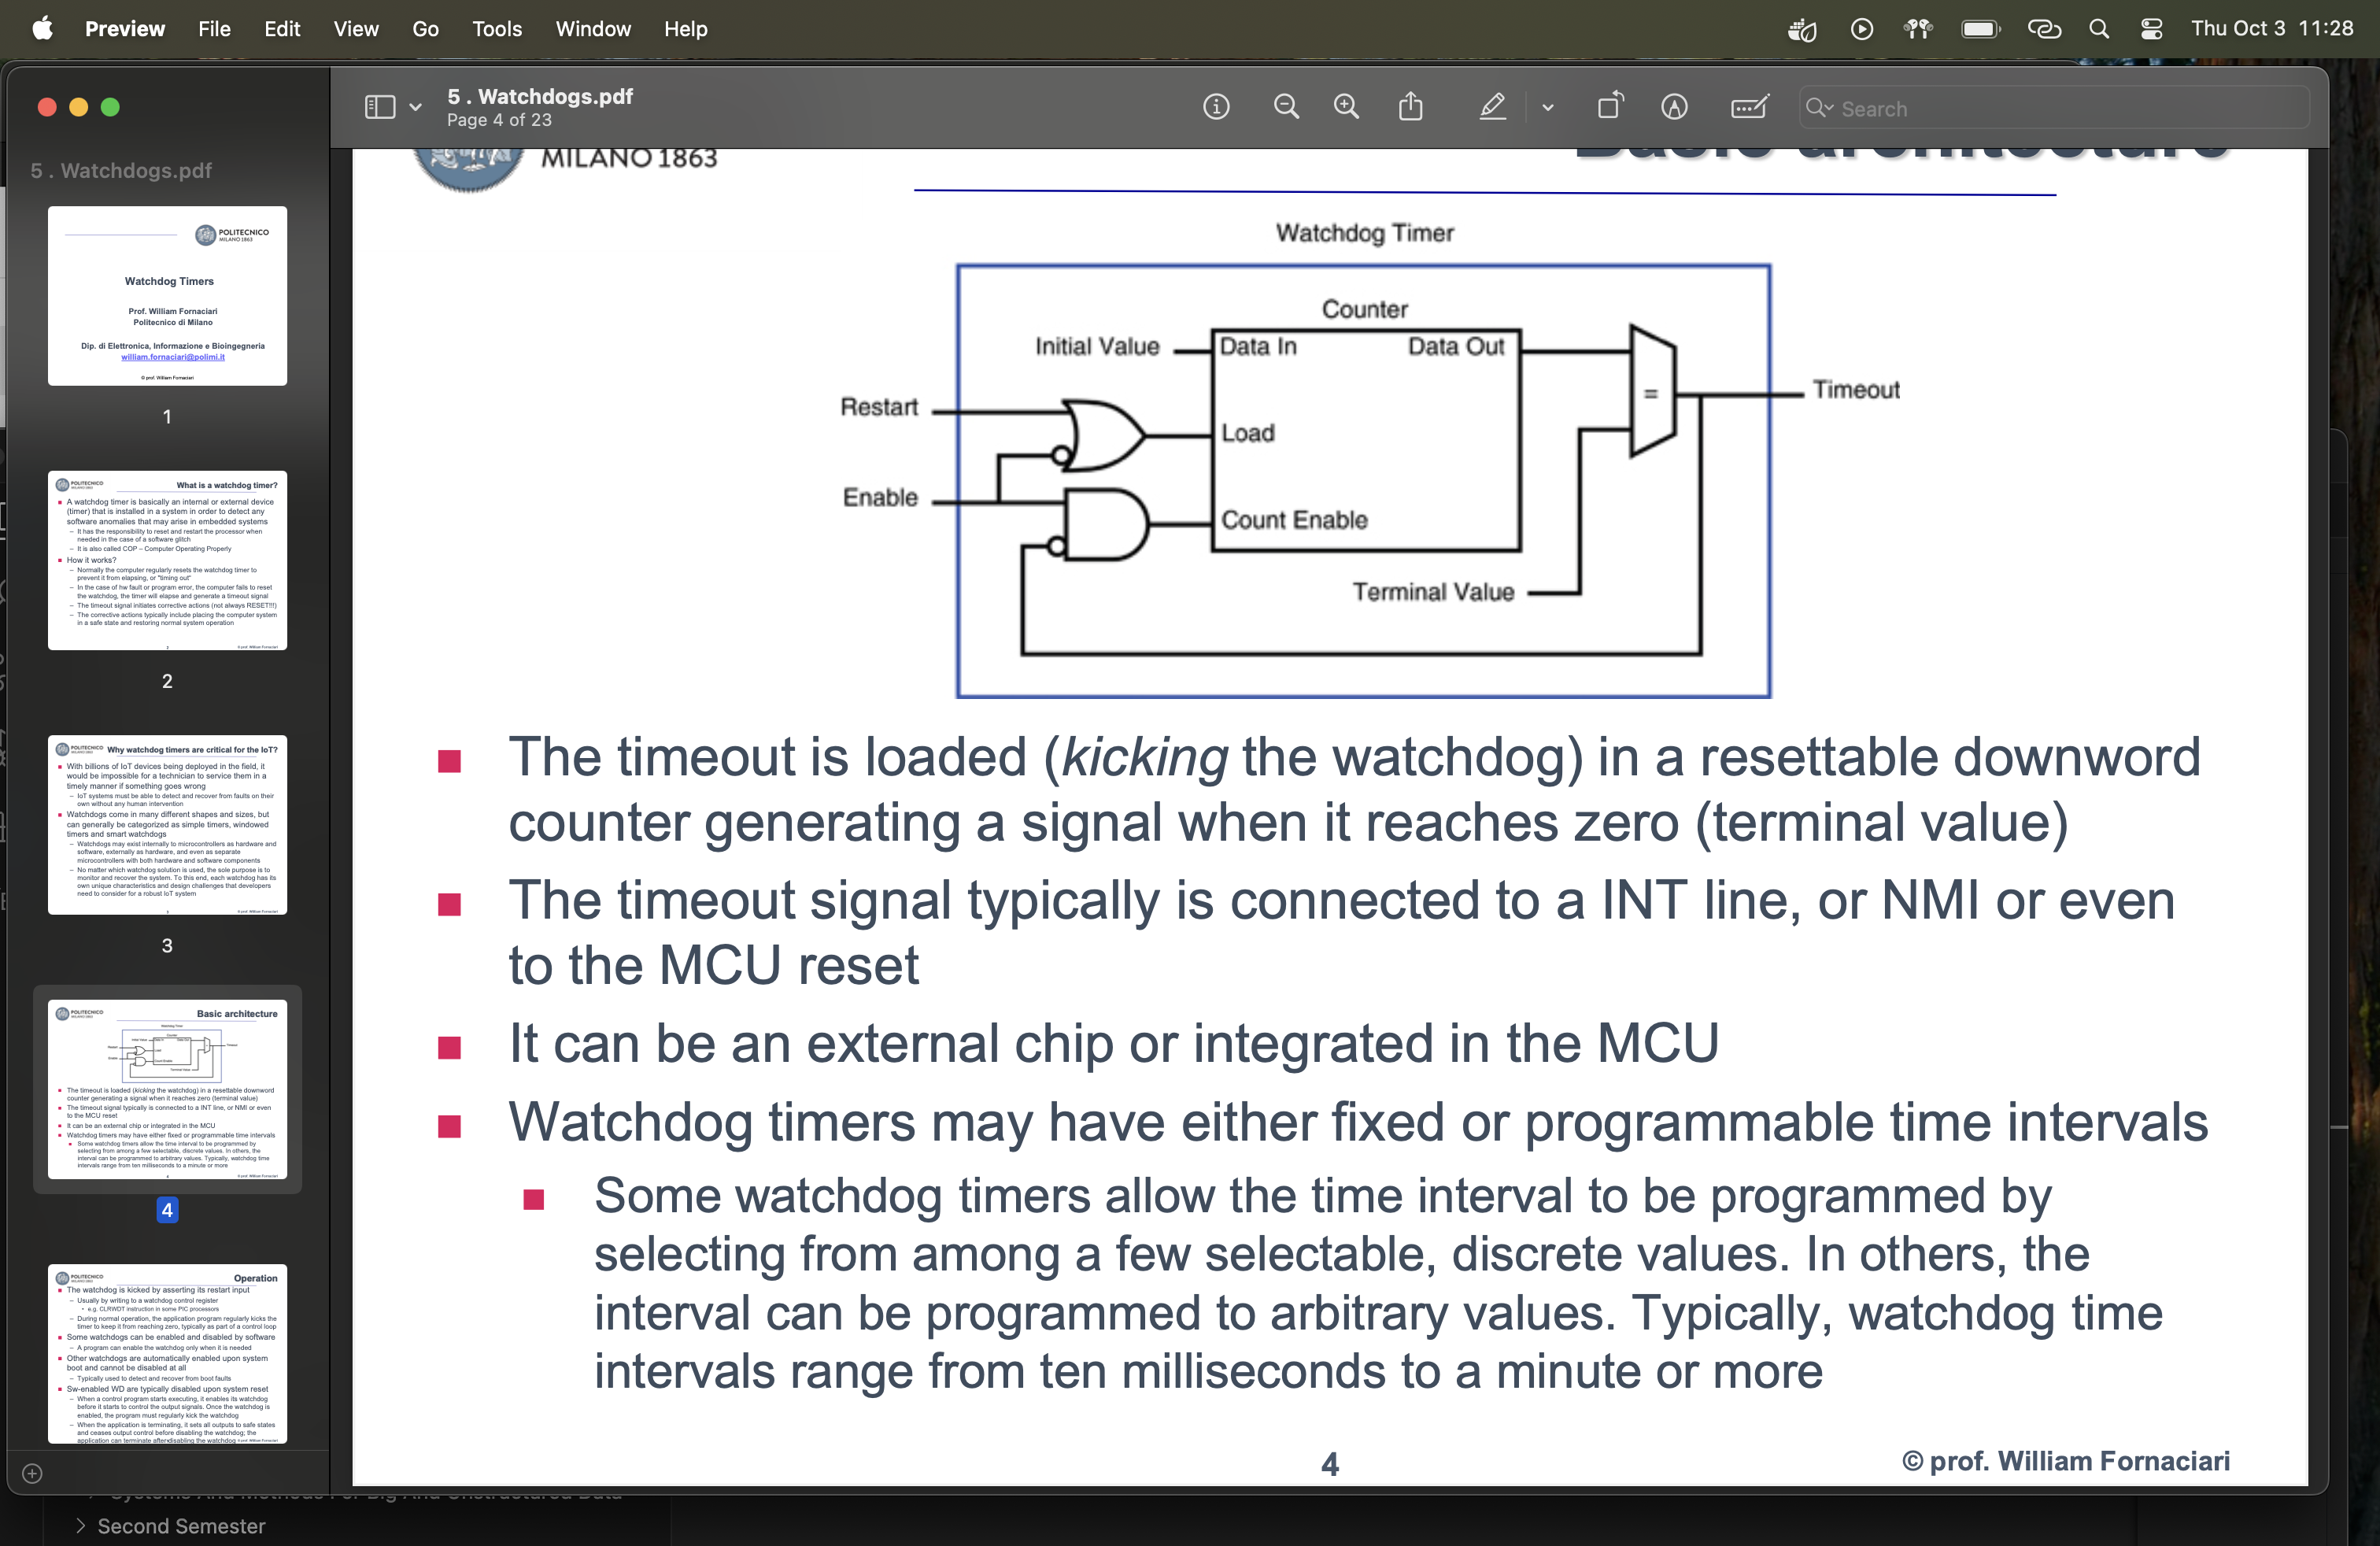
\includegraphics[width=0.75\linewidth]{images/wdog.png}
    \caption{Watchdog architecture}
\end{figure}
The watchdog timer operates as a countdown timer, which is periodically reset by the system. 
When the countdown reaches zero, a timeout signal is generated. 
While the program can modify run mode states at any time, safe mode states can only be changed through a special write mechanism. 
When the watchdog times out, the data selector switches to safe mode states.
Since the control circuitry remains operational, it retains vital state information, which may be needed for fault recovery.
\begin{figure}[H]
    \centering
    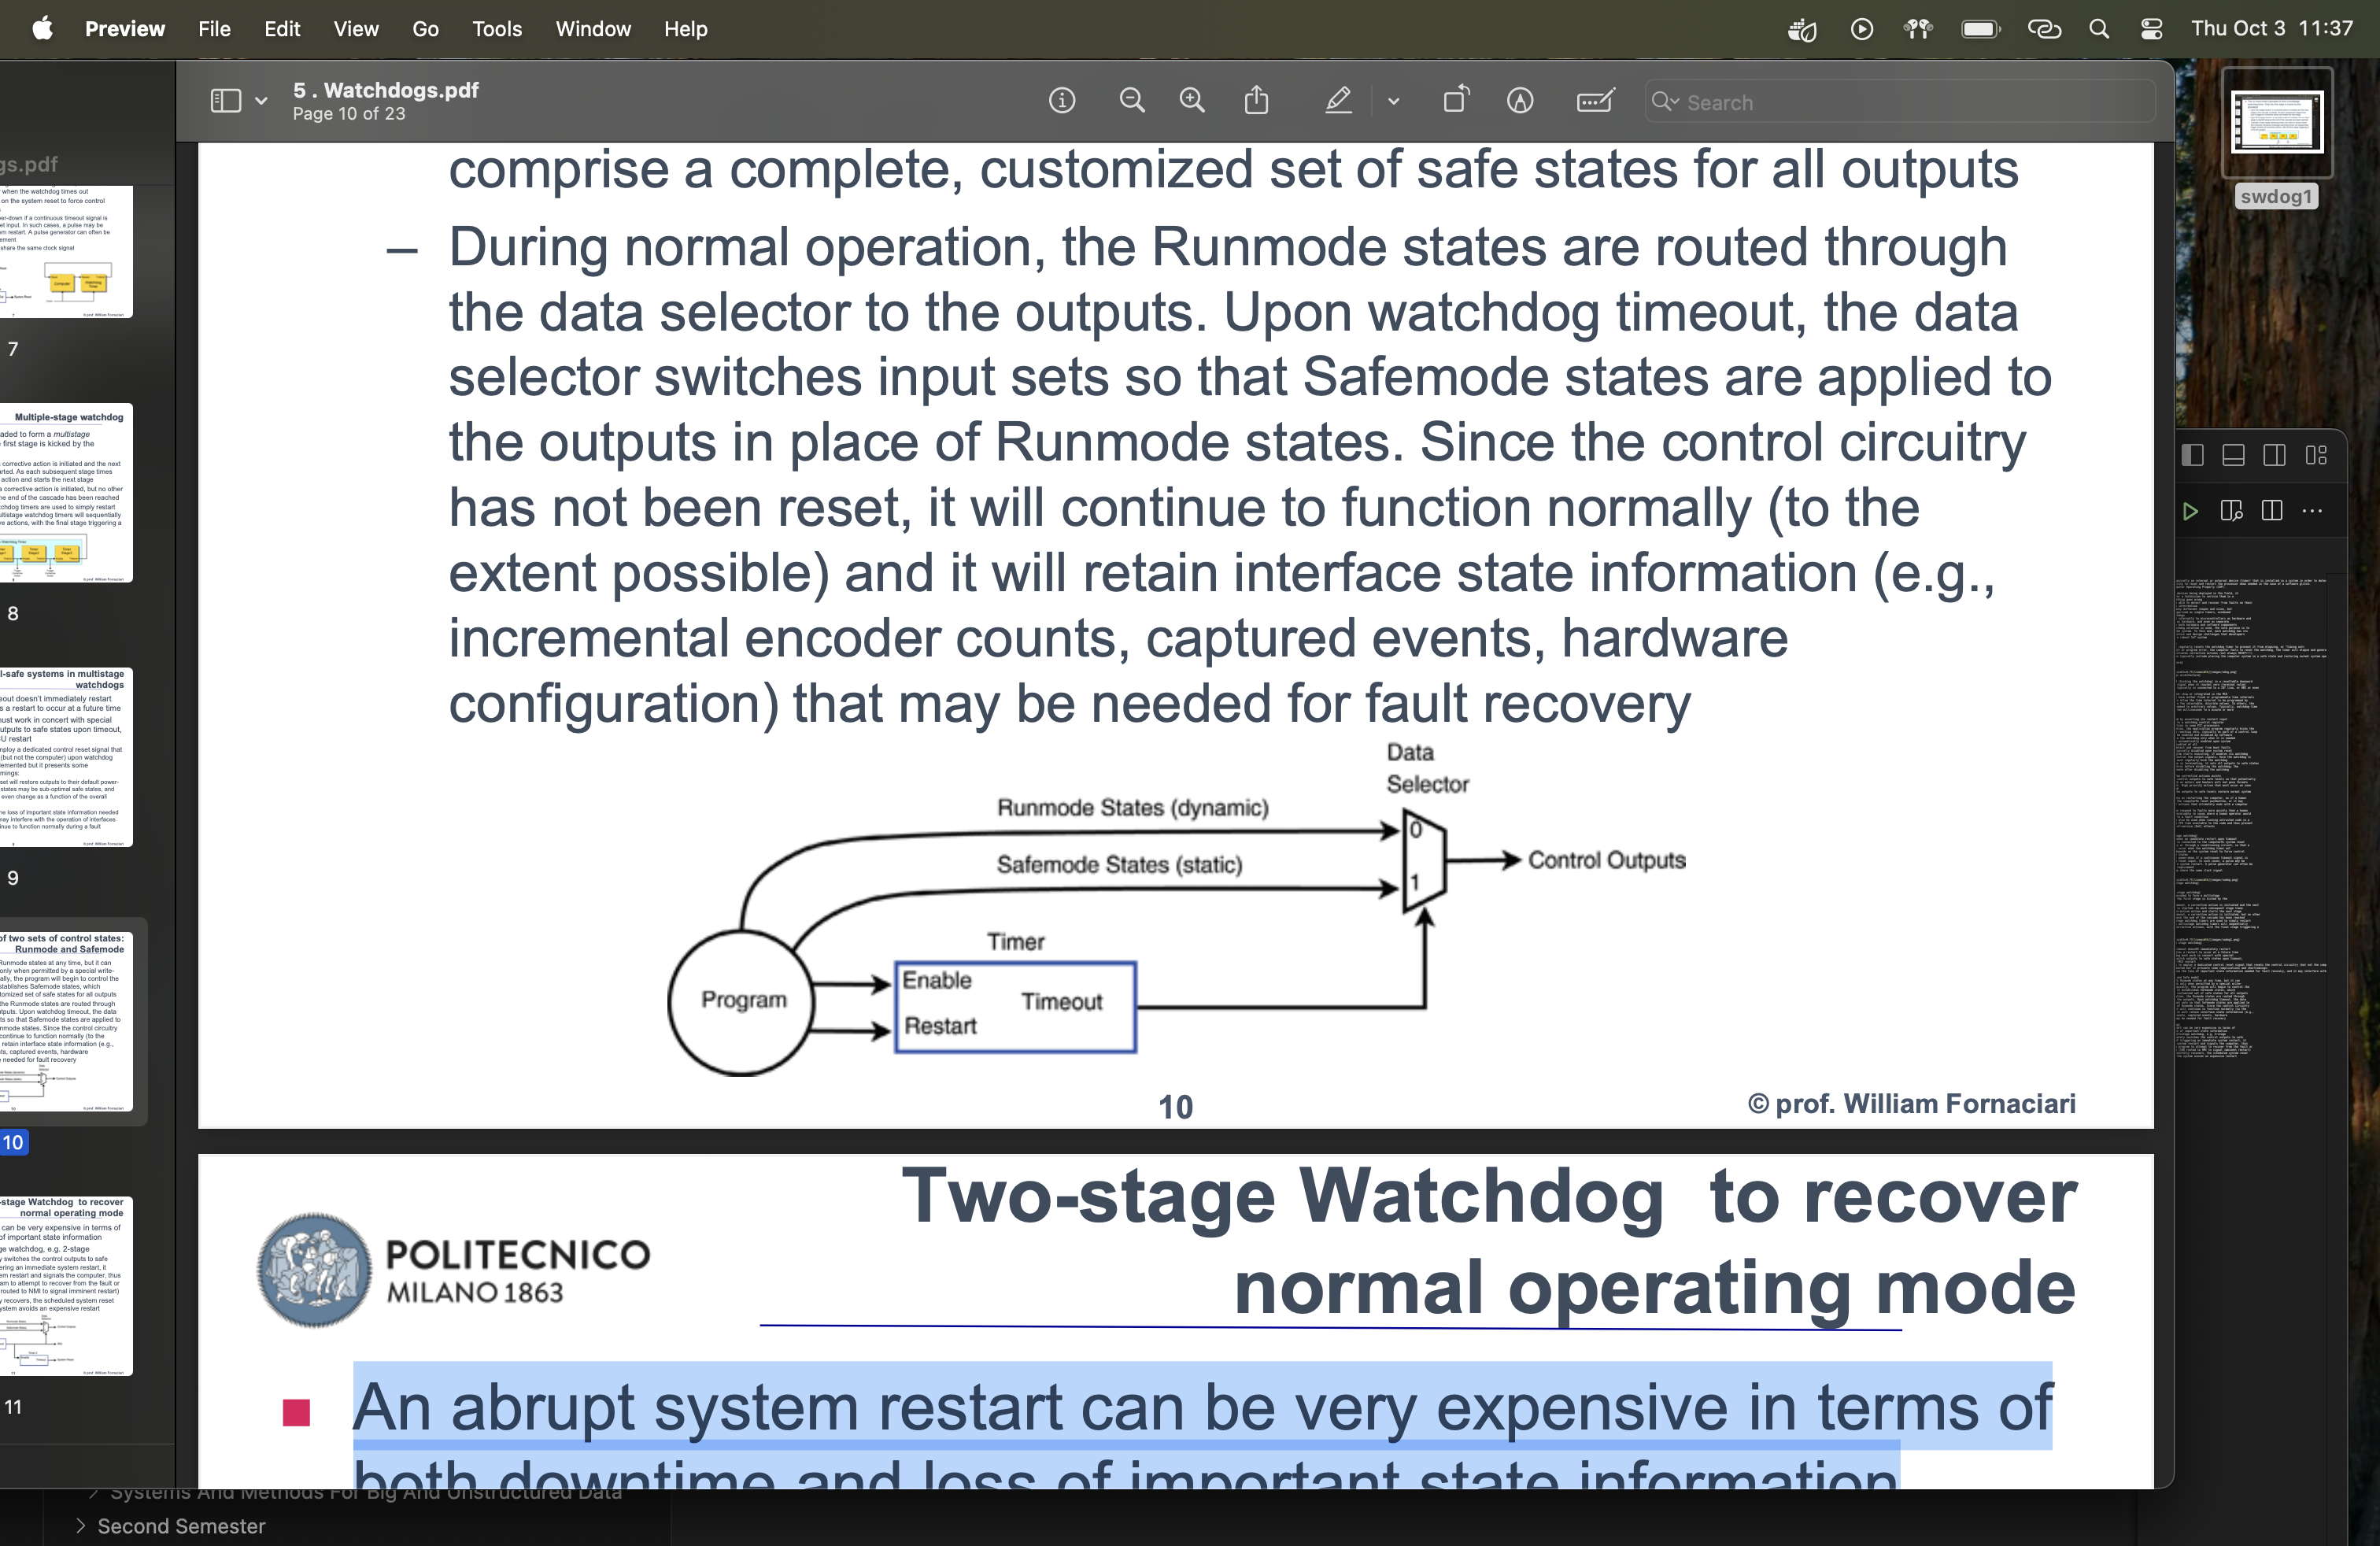
\includegraphics[width=0.75\linewidth]{images/wdog1.png}
    \caption{Watchdog mode}
\end{figure}

A system may enable the watchdog only when it is needed, while in other cases, watchdogs are automatically activated upon system boot and cannot be disabled (boot fault detection). 
When a system resets, watchdog timers are typically disabled until the control program explicitly enables them.
When the application is terminating, it should disable the watchdog after safely shutting down all outputs and stopping control operations.

When a fault is detected, the watchdog performs the following actions actions:
\begin{enumerate}
    \item \textit{Safe state transition}: the system immediately sets all control outputs to safe levels as soon as the fault is detected. 
    \item \textit{System recovery}: normal operation can be restored. 
\end{enumerate}

\paragraph*{Single stage watchdog}
A single-stage watchdog timer is a design where an immediate system restart is triggered upon timeout. 
The system relies on this reset to bring the control outputs to their safe states.
Both the microcontroller and the watchdog timer may share the same clock signal for synchronized operation.
\begin{figure}[H]
    \centering
    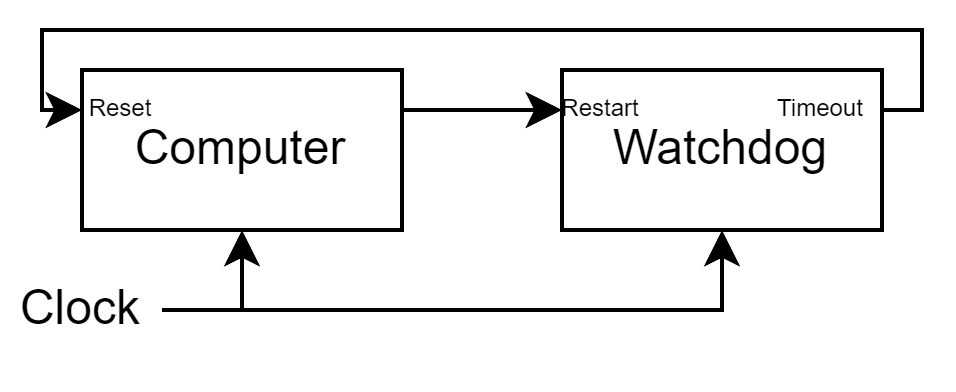
\includegraphics[width=0.5\linewidth]{images/swdog.png}
    \caption{Single stage watchdog}
\end{figure}

\paragraph*{Multiple stage watchdog}
A multi-stage watchdog consists of two or more timers arranged in a cascade. 
Only the first stage is reset by the processor, and upon its timeout, subsequent stages are initiated, each triggering corrective actions before starting the next stage.
Upon the timeout of the final stage, no further stages are initiated, and typically a full system restart is triggered.
Multi-stage watchdogs enable a series of corrective actions that happen in stages before restarting the system.
\begin{figure}[H]
    \centering
    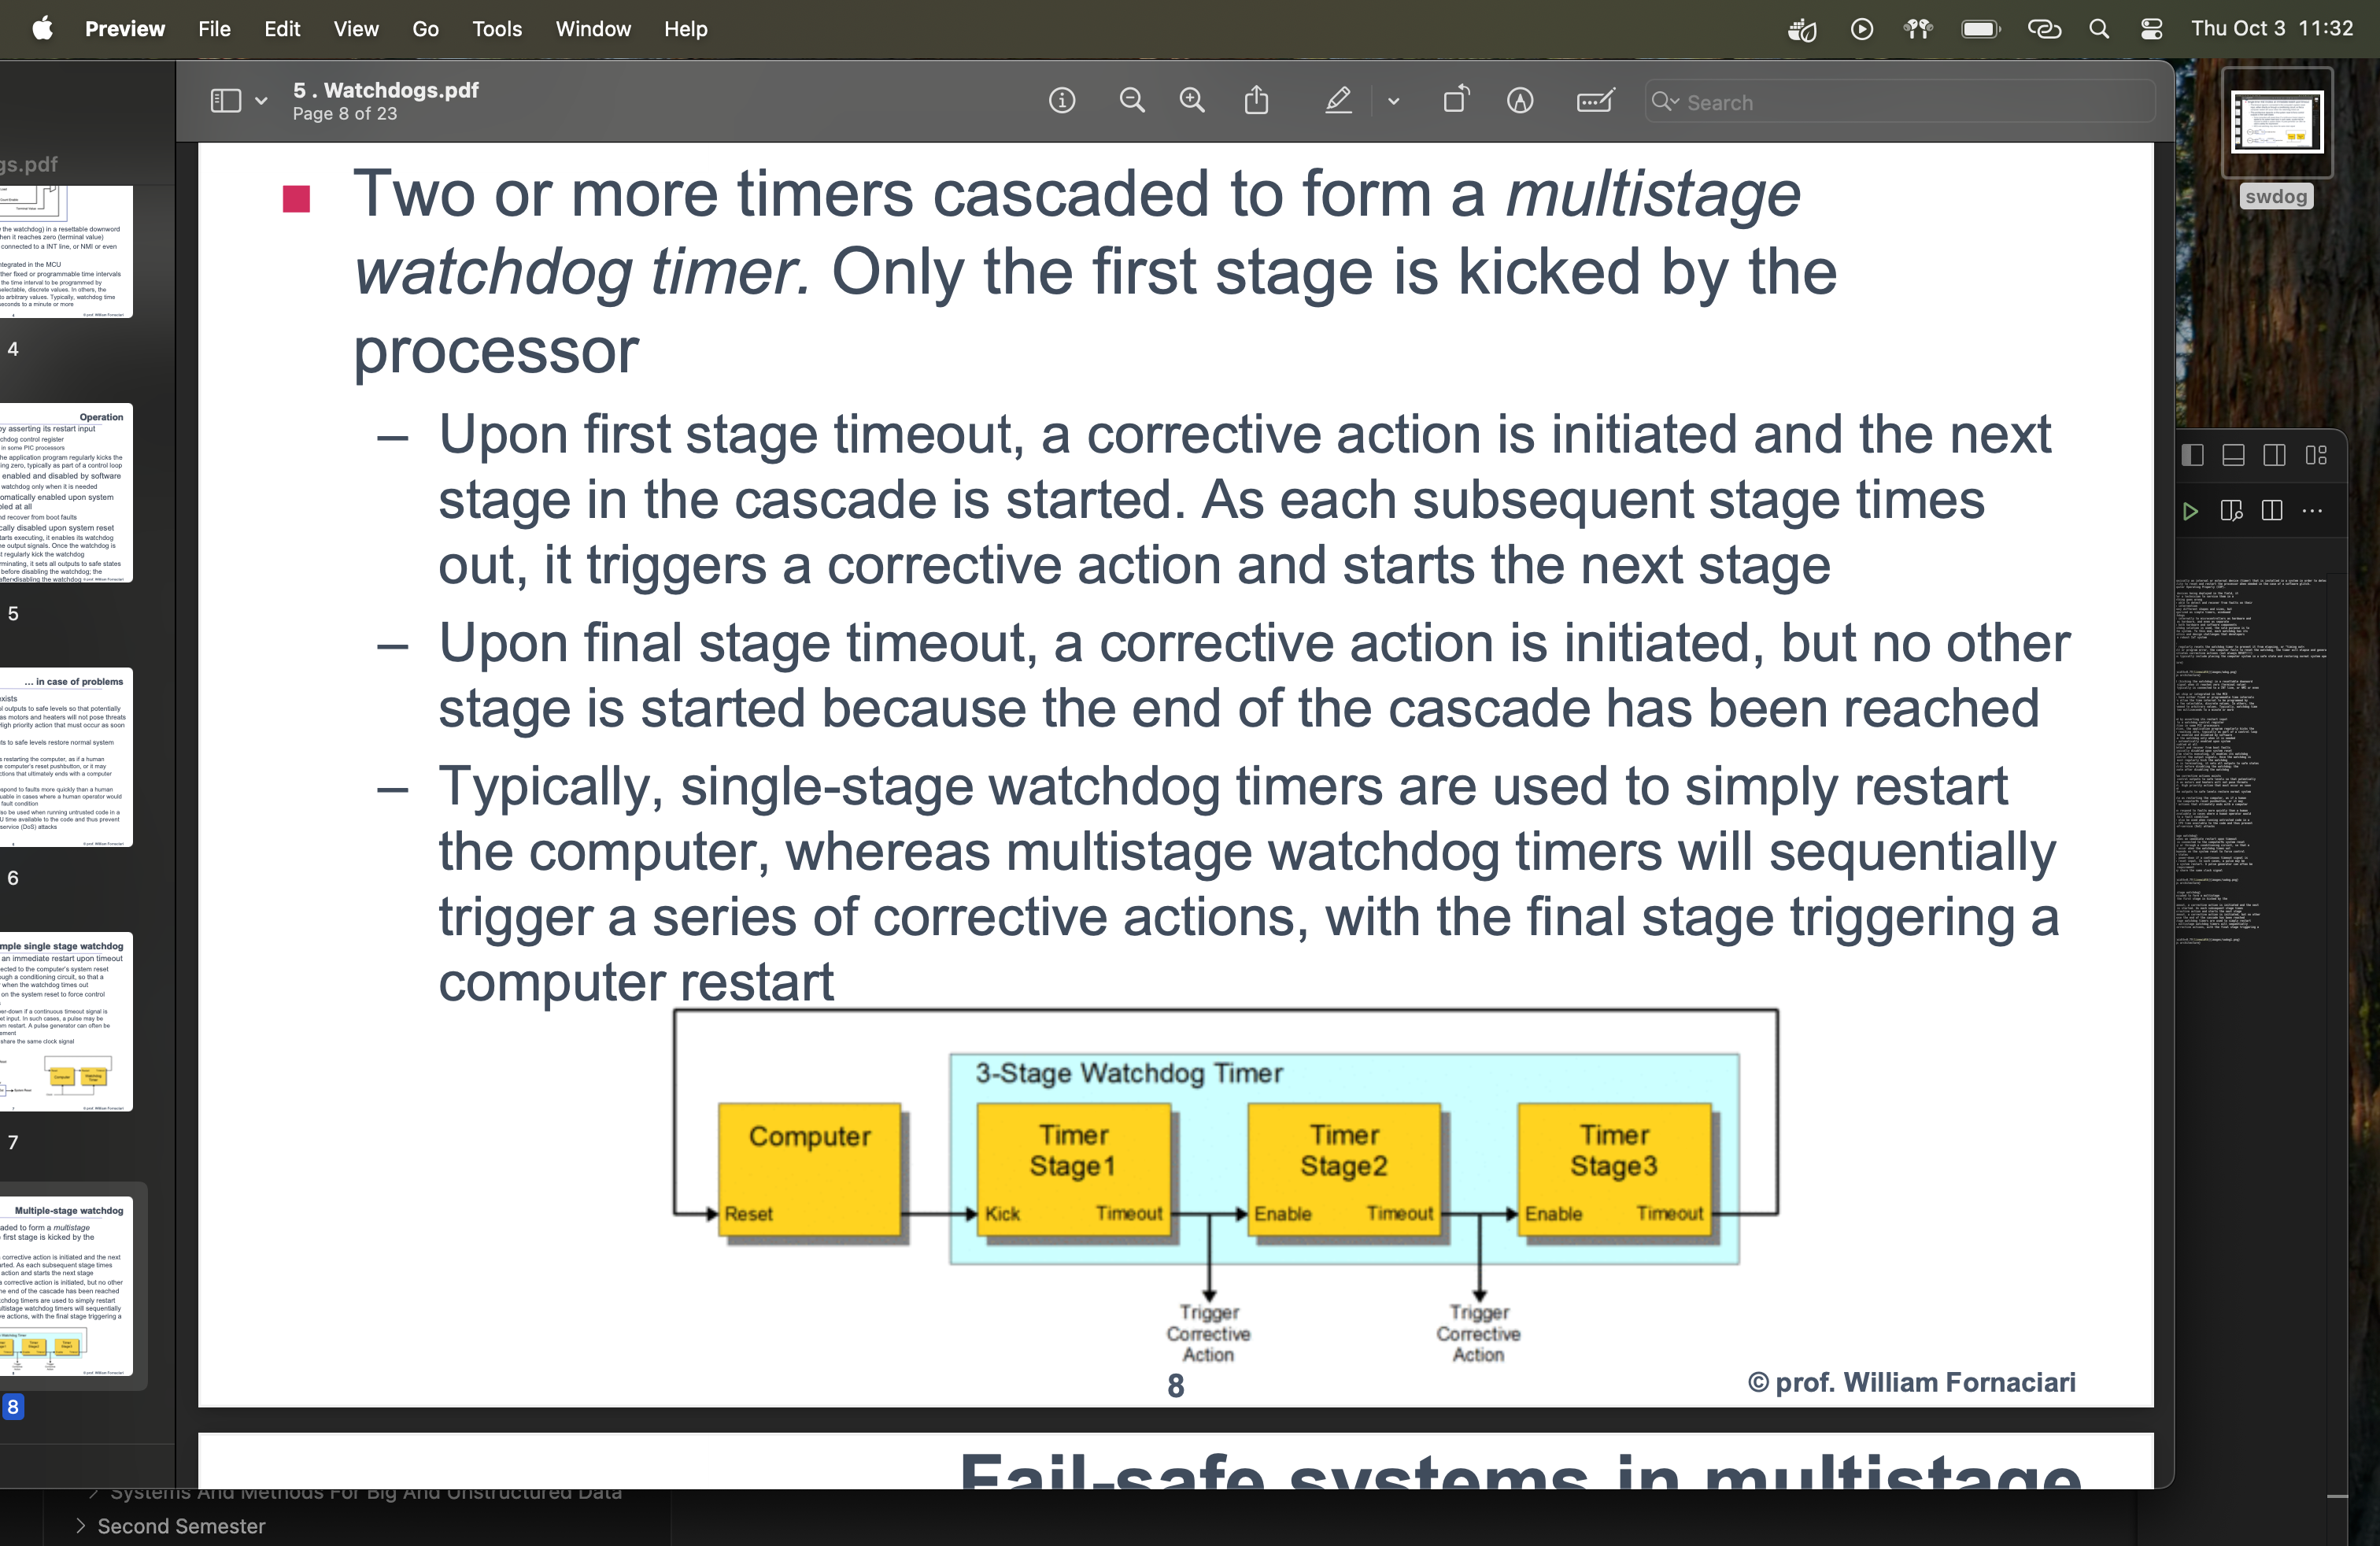
\includegraphics[width=0.75\linewidth]{images/swdog1.png}
    \caption{Multiple stage watchdog}
\end{figure}
A common technique in multiple stage designs is using a dedicated control reset signal, which resets the control circuitry without resetting the computer itself. 
Watchdog timers can trigger various corrective actions, including maskable interrupts, non-maskable interrupts, processor resets, fail-safe state activations, power cycling, depending on the system architecture.
Abrupt system restarts due to watchdog timeouts can be costly, both in terms of downtime and the potential loss of important state information. 
A multi-stage watchdog mitigates this by providing a more controlled recovery process:
\begin{enumerate}
    \item The watchdog switches control outputs to safe states immediately.
    \item The watchdog schedules a deferred restart and signals the computer, allowing the program time to attempt recovery or log critical state information.
    \item If recovery is successful, the scheduled restart can be canceled.
\end{enumerate}
\begin{figure}[H]
    \centering
    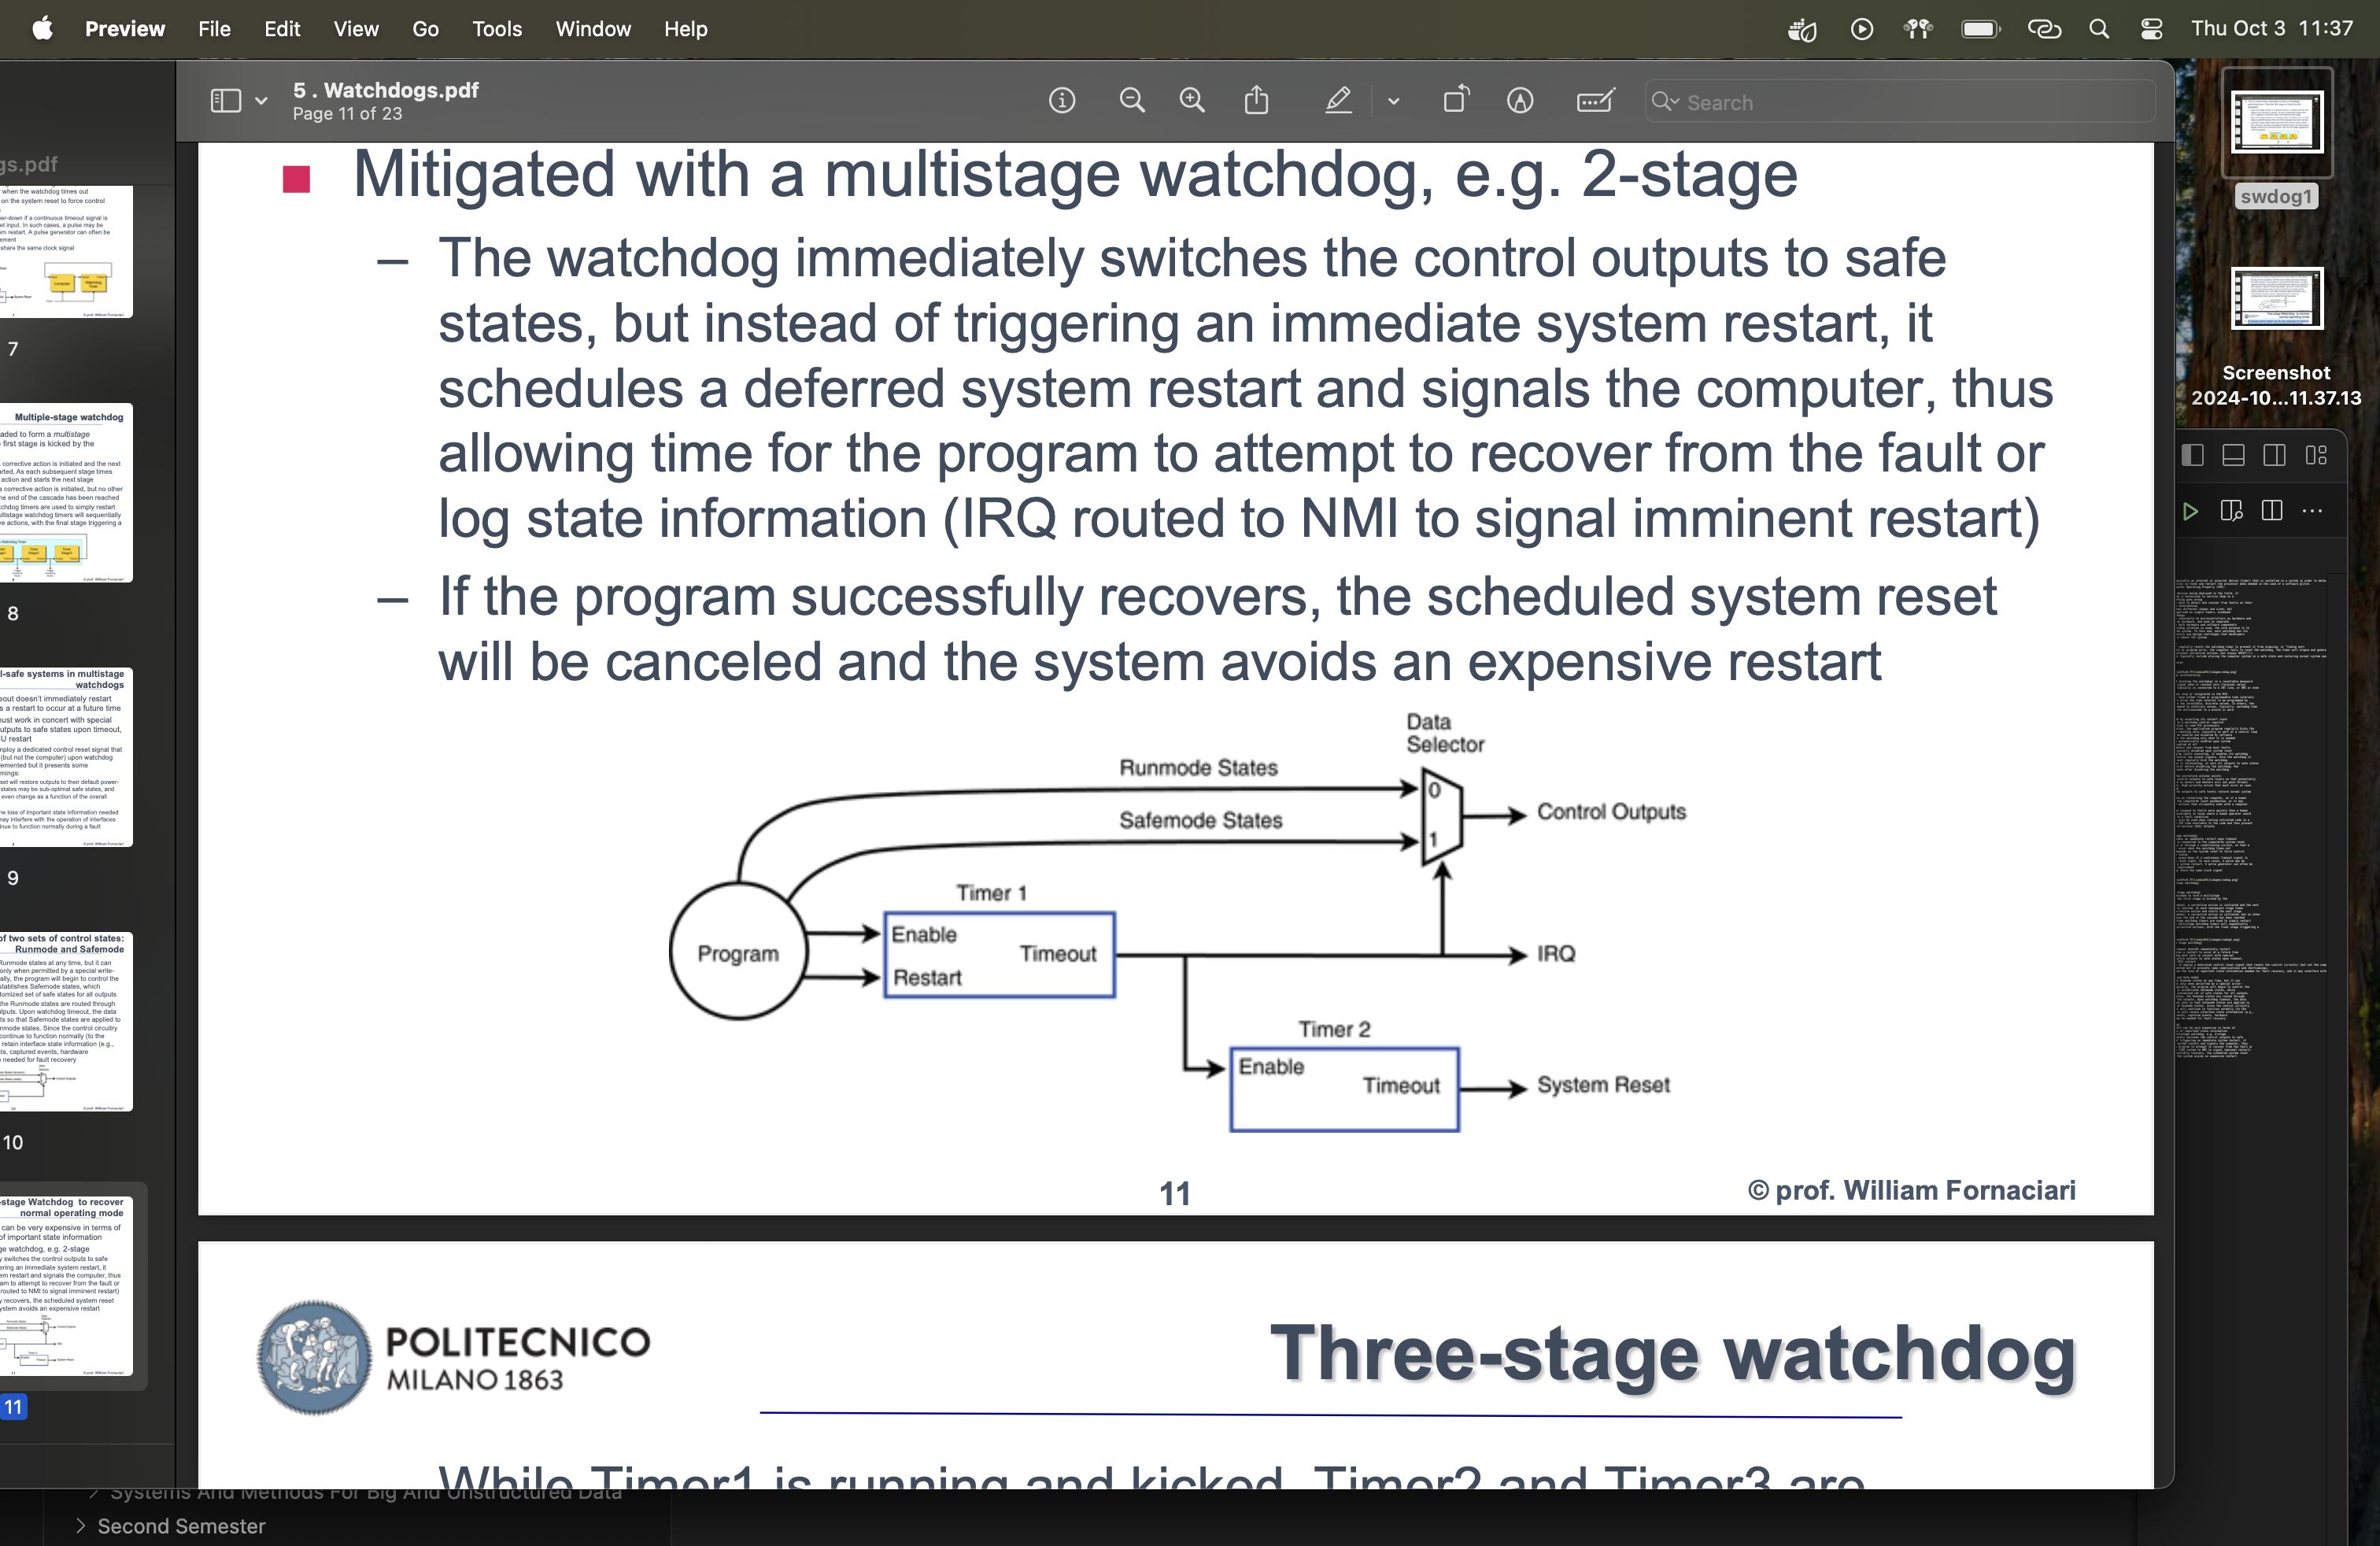
\includegraphics[width=0.75\linewidth]{images/wdog2.png}
    \caption{Watchdog recovery}
\end{figure}

\paragraph*{Taxonomy}
The main types of watchdogs are: 
\begin{itemize}
    \item \textit{AVR}: this watchdog is equipped with a special timer (WDT), which operates independently of the main system clock. 
        It acts as a counter that increments with each clock cycle from the oscillator, forcing an interrupt or a system reset once the counter reaches a pre-configured timeout value. 
        In normal operation, the application code must issue a reset (WDR) instruction to reset the counter before it reaches the timeout value.
        If this reset does not occur, the system will either generate an interrupt or trigger a system reset, depending on the selected watchdog mode.
        There are three primary modes in which this watchdog can operate:
        \begin{itemize}
            \item \textit{Interrupt} (WDTIE bit): when the watchdog timer expires, it generates an interrupt. 
            \item \textit{System reset} (WDE bit): when the watchdog timer expires, it forces a system reset. 
            \item \textit{Interrupt and system reset}: when the watchdog timer expires, an interrupt is generated first, allowing the system to save critical parameters or execute a graceful shutdown. 
                Afterward, a system reset follows to restart the system safely. 
        \end{itemize}
    \item \textit{Smart}: function as a supervisory microcontroller that monitors also system communications.
        In some cases, the microcontroller might stop responding to network commands, while still resetting the watchdog timer as usual.
        A smart watchdog addresses this by monitoring communication lines. 
    \item \textit{External}: offers several advantages that contribute to system robustness.
        This kind of watchdog provides an autonomous process to monitor the system's health, significantly increasing system reliability.
        However, the additional hardware required increases both the complexity of the system and the overall cost.
\end{itemize}

\paragraph*{Best practice}
To maximize the effectiveness of watchdog timers, several best practices should be followed. 
Disabling the watchdog for any reason should be avoided, as it opens the system to vulnerabilities. 
Additionally, clearing the watchdog timer in periodic interrupts without first performing functionality checks is a common mistake that can lead to runaway software overriding the watchdog's safety mechanism.

It's important to use an independent watchdog timer with a separate clock, allowing it to detect when the system clock has halted.
 Implementing a windowed watchdog is also recommended. 
A windowed watchdog enforces a minimum time delay before the watchdog can be reset. 
This ensures that if runaway software tries to clear the watchdog too quickly, the system will still be reset.